\section{Nichtlineare Optimierung}
\subsection{Definitionen}
  Gradient: $\overline{\grad} f = \nabla f = [f_{x_1}, f_{x_2}, \ldots, f_{x_n} ]^T$ (Spaltenvektor)
  
  Satz von Schwarz: $\frac{\partial^2 f(x_1, x_2)}{\partial x_1 \partial x_2} = \frac{\partial^2 f(x_1, x_2)}{\partial x_2 \partial x_1}$

\subsection{Gradientenverfahren}
  \begin{minipage}{14cm}
    Von der Stelle $\vec{x}^{(i)}$ wird in Richtung des Antigradienten geschritten. Die Schrittweite
    $\alpha_i$ wird bei jedem Schritt adaptiert. \todo{wie?}
    $$\vec{x}^{(i+1)} = \vec{x}^{(i)} - \alpha_i \nabla f(\vec{x}^{(i)})$$
    
    Vorteile:
    \begin{liste}
      \item Einfach zu implementieren
      \item Findet optimale Lösung
      \item Keine gute Startnäherung nötig
    \end{liste}
    
    Nachteile:
    \begin{liste}
      \item Konvergiert langsam
      \item In der Nähe der optimalen Lösung Zick-Zack-Kurs
    \end{liste}
  \end{minipage}
  \begin{minipage}{5cm}
    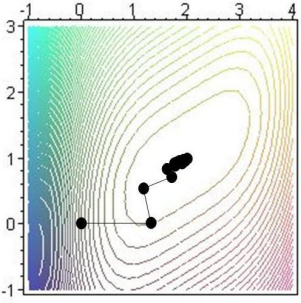
\includegraphics[width=5cm]{./Content/NonLinearOptimization/gradient-descent}
  \end{minipage}
  
\subsection{Newton-Verfahren}
  
  
  
\subsection{Quasi-Newton-Verfahren}
